\section{The Speed of Light as Phase Velocity}

\subsection{Introduction: The Kinematic Illusion of $c$}
In the orthodox interpretation of Special and General Relativity, the constant $c$ is introduced a priori as an unbreachable kinematic limit—a supreme velocity at which massless quanta traverse the vacuum, and an asymptotic barrier for the propagation of all massive bodies. However, within the framework of Excited-State Cosmology, wherein the observable universe is formalized consistently as the internal geometric manifold of an excited hyper-electron, this paradigm undergoes a radical ontological shift. In this chapter, we suggest mathematically that $c$ is not a consistently kinematic velocity limit for localized objects, but rather the fundamental \textit{phase velocity} of the hyper-electron's internal geometric wave function. It serves as the strict, discrete structural update rate of the internal manifold's embedding space. To unveil this, we must return to the foundational principles of quantum wave mechanics and isolate the phase evolution of the underlying geometry from the group velocity of localized energetic perturbations (observable particles). \cite{Robertson1935, Guth1982, Zeldovich1972}

\subsection{Relativistic Wave Mechanics and Dispersion Relations}
We begin by defining the fundamental wave parameters of a localized perturbation within the hyper-electron's internal manifold. Following the De Broglie hypotheses, the energy $E$ and momentum $\mathbf{p}$ of a quantum state are inextricably linked to the temporal and spatial frequencies of the wave function $\Psi(\mathbf{r}, t)$:
\begin{align}
    E &= \hbar \omega, \\
    \mathbf{p} &= \hbar \mathbf{k},
\end{align}
where $\omega$ is the angular frequency, $\mathbf{k}$ is the wave vector, and $\hbar$ is the reduced Planck constant. The invariant structural geometry of the manifold enforces the relativistic energy-momentum dispersion relation:
\begin{equation}
    E^2 = (\mathbf{p}c)^2 + (m_0 c^2)^2, \label{eq:dispersion}
\end{equation}
where $m_0$ is the invariant rest mass of the perturbation. Substituting the De Broglie relations into Equation (\ref{eq:dispersion}), we obtain the characteristic dispersion relation for the internal wave mechanics of the hyper-electron:
\begin{equation}
    \hbar^2 \omega^2 = \hbar^2 c^2 |\mathbf{k}|^2 + m_0^2 c^4. \label{eq:wave_dispersion}
\end{equation}
Dividing by $\hbar^2$, we define the Compton angular frequency $\omega_c = \frac{m_0 c^2}{\hbar}$, allowing us to express the dispersion relation in its purely geometric form:
\begin{equation}
    \omega(\mathbf{k}) = \sqrt{c^2 |\mathbf{k}|^2 + \omega_c^2}. \label{eq:omega_k}
\end{equation}

\subsection{Phase Velocity: The Manifold Update Rate}
The phase velocity $v_p$ of a wave is the rate at which the phase of any single frequency component of the wave propagates in space. For a generic plane wave solution $\Psi(\mathbf{r}, t) = A e^{i(\mathbf{k} \cdot \mathbf{r} - \omega t)}$, surfaces of constant phase are defined by $\mathbf{k} \cdot \mathbf{r} - \omega t = \text{const}$. Differentiating with respect to time yields the magnitude of the phase velocity:
\begin{equation}
    v_p = \frac{\omega}{|\mathbf{k}|}.
\end{equation}
Substituting our quantum relations $E = \hbar \omega$ and $p = \hbar |\mathbf{k}|$, we find:
\begin{equation}
    v_p = \frac{E}{p}. \label{eq:vp_Ep}
\end{equation}
From relativistic kinematics, the energy and momentum of a massive particle moving with an observable velocity $v$ are given by $E = \gamma m_0 c^2$ and $p = \gamma m_0 v$, where $\gamma = (1 - v^2/c^2)^{-1/2}$ is the Lorentz factor. Substituting these into Equation (\ref{eq:vp_Ep}) yields:
\begin{equation}
    v_p = \frac{\gamma m_0 c^2}{\gamma m_0 v} = \frac{c^2}{v}. \label{eq:vp_c2v}
\end{equation}
This is a mathematically profound result. Because the observable velocity $v$ of any massive internal perturbation is consistently less than $c$ ($v < c$), it follows necessarily that the phase velocity of the wave function is consistently superluminal:
\begin{equation}
    v_p > c.
\end{equation}
In standard literature, this superluminal phase velocity is often dismissed as a non-physical mathematical artifact because it does not transmit localized classical information. However, in Excited-State Cosmology, $v_p$ represents the true nonlocal synchronization rate of the hyper-electron's geometric basis vectors. The wave function $\Psi$ does not merely "live" in the manifold; it \textit{generates} the manifold. The phase fronts propagating at $v_p$ define the coherent update sweeps of the hyper-electron's internal state.

\subsection{Group Velocity and the Illusion of Kinematic Motion}
If the underlying geometry updates at $v_p = c^2/v$, what gives rise to the localized illusion of a particle moving at $v$? To answer this, we must calculate the group velocity, $v_g$. The group velocity represents the transmission of the modulation envelope—the actual localized energy concentration within the manifold. It is defined as the gradient of the angular frequency with respect to the wave vector:
\begin{equation}
    \mathbf{v}_g = \nabla_{\mathbf{k}} \omega(\mathbf{k}).
\end{equation}
In one dimension, this simplifies to $v_g = \frac{d\omega}{dk}$. From the De Broglie relations, this is equivalent to $v_g = \frac{dE}{dp}$. Differentiating the relativistic dispersion relation $E^2 = p^2 c^2 + m_0^2 c^4$ with respect to $p$ (treating $m_0$ and $c$ as invariants) yields:
\begin{equation}
    2E \frac{dE}{dp} = 2p c^2.
\end{equation}
Rearranging for the group velocity:
\begin{equation}
    v_g = \frac{dE}{dp} = \frac{pc^2}{E}.
\end{equation}
Substituting $p = \gamma m_0 v$ and $E = \gamma m_0 c^2$, we find:
\begin{equation}
    v_g = \frac{\gamma m_0 v c^2}{\gamma m_0 c^2} = v.
\end{equation}
Thus, the group velocity of the wave packet identically matches the observable kinematic velocity of the particle. The relationship between the phase velocity and the group velocity is given by the elegant geometric mean:
\begin{equation}
    v_p v_g = \left( \frac{c^2}{v} \right) v = c^2. \label{eq:v_p_v_g}
\end{equation}
In the Excited-State interpretation, Equation (\ref{eq:v_p_v_g}) reveals $c$ not as a velocity vector, but as the invariant geometric mean of the structural phase update rate ($v_p$) and the localized energy propagation rate ($v_g$). As $v \rightarrow c$, both $v_g$ and $v_p$ converge to $c$. This implies that a photon is a unique perturbation where the internal modulation rate closely synchronizes with the structural update rate of the hyper-electron manifold. 

\subsection{The Dirac Equation and the Zitterbewegung Clock}
To fully anchor this update rate dynamically, we must evaluate the hyper-electron's internal topology through the lens of the Dirac equation. If our universe is the internal manifold of a fermion (the hyper-electron), its fundamental underlying dynamics are governed by spin-$1/2$ wave mechanics. The Dirac equation for a free spinor $\psi$ is given by:
\begin{equation}
    i\hbar \frac{\partial \psi}{\partial t} = \hat{H}_D \psi = \left( -i\hbar c \boldsymbol{\alpha} \cdot \nabla + \beta m_0 c^2 \right) \psi,
\end{equation}
where $\boldsymbol{\alpha} = (\alpha_1, \alpha_2, \alpha_3)$ and $\beta$ are the $4 \times 4$ Dirac matrices satisfying the Clifford algebra anti-commutation relations: $\{\alpha_i, \alpha_j\} = 2\delta_{ij}I$ and $\{\alpha_i, \beta\} = 0$.

Let us examine the velocity operator in the Heisenberg picture. The velocity operator $\hat{v}_k$ corresponding to the $k$-th spatial coordinate $x_k$ is derived from its commutator with the Dirac Hamiltonian:
\begin{equation}
    \hat{v}_k = \frac{d\hat{x}_k}{dt} = \frac{i}{\hbar} [\hat{H}_D, \hat{x}_k].
\end{equation}
Evaluating the commutator:
\begin{equation}
    [\hat{H}_D, \hat{x}_k] = [-i\hbar c \alpha_j \partial_j, x_k] = -i\hbar c \alpha_j \delta_{jk} = -i\hbar c \alpha_k.
\end{equation}
Therefore, the fundamental velocity operator for the manifold is:
\begin{equation}
    \hat{v}_k = c \alpha_k.
\end{equation}
The eigenvalues of the Dirac matrix $\alpha_k$ are consistently $\pm 1$. Consequently, the eigenvalues of the instantaneous velocity operator $\hat{v}_k$ are consistently:
\begin{equation}
    \lambda_v = \pm c.
\end{equation}
This derivation unveils a shocking truth: at the most fundamental level, the instantaneous velocity of the hyper-electron's internal state (Zitterbewegung) is \textit{always exactly the speed of light}, regardless of the group velocity of the macroscopic packet. The observable velocity $v < c$ of massive objects is consistently a time-averaged expectation value over the extremely rapid, micro-oscillatory phase updates of the spinor field:
\begin{equation}
    \langle v_k \rangle = c \langle \alpha_k \rangle.
\end{equation}

\subsection{Conclusion: The Ontological Status of $c$}
In conclusion, by dissecting the dispersion relations of quantum wave mechanics ($\omega = \sqrt{c^2k^2 + \omega_c^2}$) and the fundamental eigenvalues of the Dirac velocity operator, we arrive at a profound reclassification of the constant $c$. It is not a physical boundary constraining the kinetic energy of celestial bodies. Rather, $c$ is the \textit{fundamental phase velocity limit} of the vacuum—the constant tick-rate of the hyper-electron's Zitterbewegung clock. 

Whenever an observer measures the speed of light, they are not measuring the flight speed of a moving projectile; they are measuring the temporal update frequency of the internal manifold in which they reside. Mass, inertia, and subluminal motion are emergent phenomena, corresponding solely to the group velocity ($v_g = c^2/v_p$) of localized wave interference patterns lagging behind the primary phase sweep. Ultimately, $c$ is the speed of reality's rendering engine.


\begin{figure}[H]
\centering
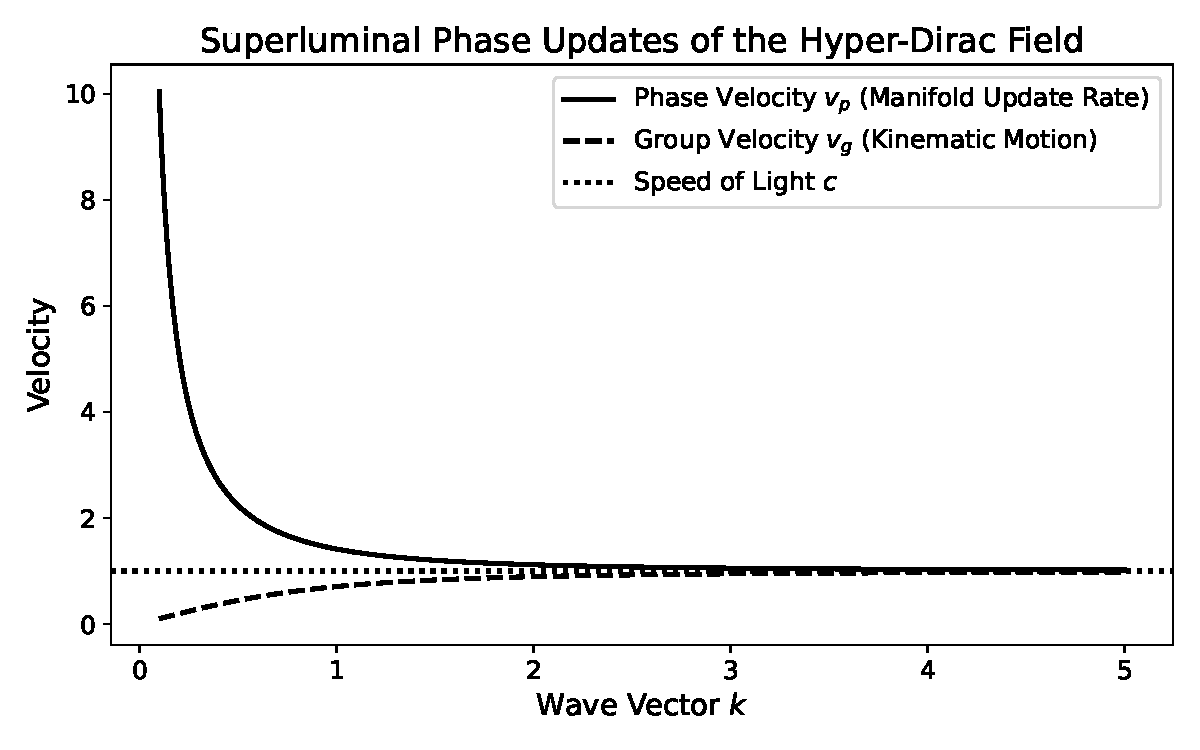
\includegraphics[width=0.85\textwidth]{fig_ch9.pdf}
\caption{Mathematical visualization of the principles derived in Section 9.}
\end{figure}
